%
% Assignment Template v19.02
%
%%% 20xx0x/MATHxxx/Crowdmark/Ax
%
\documentclass[12pt]{article} %
\usepackage{amsthm}
\usepackage{CKpreamble}
\usepackage{CKassignment}
\usepackage{mdframed}
\usepackage{enumitem}
\usepackage{import}
\usepackage{pdfpages}
\usepackage{transparent}
\usepackage{xcolor}
\usepackage{tkz-euclide}
\usepackage{physunits}
\usepackage{physics}
\usepackage{lmodern}
\usepackage{microtype}
\usepackage{euscript}
\usepackage{upgreek}
\usepackage[misc]{ifsym}
\usepackage{pdfpages}
\usepackage{euscript}
\usepackage{transparent}
\usepackage{xcolor}
\usepackage{tasks}
\usepackage{tkz-euclide}

%%% Maths and science packages

\usepackage{amsmath,amsthm,amssymb}
\usepackage{pgfplots}
	\usetikzlibrary{
		calc,
		patterns,
		positioning
	}
	\pgfplotsset{
		compat=1.16,
		samples=200,
		clip=false,
		my axis style/.style={
			axis x line=middle,
			axis y line=middle,
			legend pos=outer north east,
			axis line style={
				->,
			},
			legend style={
				font=\footnotesize
			},
			label style={
				font=\footnotesize
			},
			tick label style={
				font=\footnotesize
			},
			xlabel style={
				at={
					(ticklabel* cs:1)
				},
				anchor=west,
				font=\footnotesize,
			},
			ylabel style={
				at={
					(ticklabel* cs:1)
				},
				anchor=west,
				font=\footnotesize,
			},
			xlabel= $x$,
			ylabel=$\vec d (\m \tx{[East]})$
		},
	}
	\tikzset{
		>=stealth
	}

%%% Tables and figures packages

\usepackage{float}
\usepackage{caption}
	\captionsetup{
		format=plain,
		labelfont=bf,
		font=small,
		justification=centering
	}
	


\theoremstyle{ex}
\newtheorem*{ex}{Example}

\newcommand{\incfig}[2][1]{%
    \def\svgwidth{#1\columnwidth}
    \import{./figures/}{#2.pdf_tex}
}

\pdfsuppresswarningpagegroup=1

\newcounter{step}[section]
\newenvironment{step}[1][]
{\refstepcounter{step} \textbf{Step #1.}}


%
\begin{document}
	\pagenumbering{arabic}
	% Start of class settings ...
	\renewcommand*{\coursecode}{MATH 235} % renew course code
	\renewcommand*{\assgnnumber}{Assignment 1} % renew assignment number
	\renewcommand*{\submdate}{September 14, 2021} % renew the date
	\renewcommand*{\studentfname}{Abdullah} % Student first name
	\renewcommand*{\studentlname}{Zubair} % Student last name
    \renewcommand*{\proofname}{Proof:}
	% \renewcommand*{\studentnum}{20836288} % Student number

	\renewcommand\qedsymbol{$\blacksquare$}
	\setfigpath
	% End of class settings	
	% \pagestyle{crowdmark}
	\newgeometry{left=18mm, right=18mm, top=22mm, bottom=22mm} % page is set to default values
	\fancyhfoffset[L,O]{0pt} % header orientation fixed
	% End of class settings
	%%% Note to user:
	% CTRL + F <CHANGE ME:> (without the angular brackets) in CKpreamble to specify graphics paths accordingly.
	% The command \circled[]{} accepts one optional and one mandatory argument.
	% Optional argument is for the size of the circle and mandatory argument is for its contents.
	% \circled{A} produces circled A, with size drawn for letter A. \circled[TT]{A} produces circled A with size drawn for TT.
	% https://github.com/CalvinKent/My-LaTeX
	%%%

	%%%%%%%%%%%%%%%%%%%%%%%%%%%%%%%%%%%%%%%%%%%%%%%%%%%%%%%%%%%%%%%%%%%%%%%%%%%%%%%
	%%%                        CUSTOM MACRO VIM-TEX                             %%%
	%%       call IMAP('NOM', '\nomenclature{}', 'tex')               

	%%%%%%%%%%%%%%%%%%%%%%%%%%%%%%%%%%%%%%%%%%%%%%%%%%%%%%%%%%%%%%%%%%%%%%%%%%%%%%%

	% Crowdmark assignment start
	% qnumber, qname, qpoints

\begin{center}
		\Huge{\underline{\textbf{Solutions - Lecture 8 - Homework}}}
\end{center}
\begin{qstn} \text{ }
  \begin{itemize} 
    \item[\textit{Q3.}]
      \[
          \sin \theta = \frac{4}{5} \hspace{0.7cm} \cos \theta = \frac{3}{5} \hspace{0.7cm} \tan \theta =
          \frac{4}{3}
      .\] 

      \[
          \csc \theta = \frac{5}{4} \hspace{0.7cm} \sec \theta = \frac{5}{3} \hspace{0.7cm} \cot \theta =
          \frac{3}{4}
      .\] 

    \item[\textit{Q6.}]
      \[
          \sin \theta = \frac{15}{17} \hspace{0.7cm} \cos \theta = \frac{8}{17} \hspace{0.7cm} \tan \theta =
          \frac{15}{8}
      .\] 

      \[
          \csc \theta = \frac{17}{15} \hspace{0.7cm} \sec \theta = \frac{17}{8} \hspace{0.7cm} \cot \theta =
          \frac{8}{15}
      .\] 

    \item[\textit{Q8.}]
      \[
          \sin \theta = \frac{7}{8} \hspace{0.7cm} \cos \theta = \frac{\sqrt{15}}{8} \hspace{0.7cm} \tan \theta =
          \frac{7}{\sqrt{15}}
      .\] 

      \[
          \csc \theta = \frac{8}{7} \hspace{0.7cm} \sec \theta = \frac{8}{\sqrt{15}} \hspace{0.7cm} \cot \theta =
          \frac{\sqrt{15}}{7}
      .\] 
  \end{itemize}
\end{qstn}

\begin{qstn} \text{ }
  \begin{itemize} 
    \item[\textit{Q9a).}]
      \[
          \sin \alpha = \frac{3}{\sqrt{34}} \hspace{0.7cm} \cos \beta = \frac{3}{\sqrt{34}}
      .\] 

    \item[\textit{Q10a).}]
      \[
          \sin \alpha = \frac{4}{7} \hspace{0.7cm} \cos \beta = \frac{4}{7}
      .\] 
  \end{itemize}
\end{qstn}


\begin{qstn} \text{ }
  \begin{itemize} 
    \item[\textit{Q11.}] $x = 25 / 2$.

    \item[\textit{Q12.}] $x = 12\sqrt{2}$.

    \item[\textit{Q13.}] $x = (13\sqrt{3})/ 2$.

    \item[\textit{Q14.}] $x = 4\sqrt{3}$.

    \item[\textit{Q16.}] $x = 31.30339$.

  \end{itemize}
\end{qstn}

\newpage

\begin{qstn} \text{ }
  \begin{enumerate}[label=(\alph*)]
    \item $11 / 12$.
    \item $1$. 
    \item $3 / 2$.
    \item $22 / 3$.
  \end{enumerate}
\end{qstn}

\begin{qstn} \text{ }
  \begin{itemize} 
    \item[\textit{Q31.}]  \text{ } 
      \begin{center}
          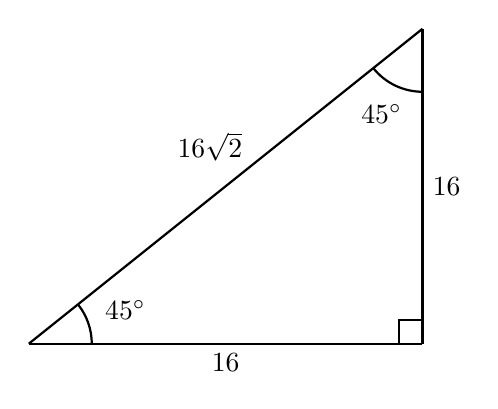
\begin{tikzpicture}[thick]
          \coordinate (A) at (0,1);
          \coordinate (B) at (5,5);
          \coordinate (C) at (5,1);

          \draw[black] (C) -- (B) node[midway, right]{$16$};
          \draw[black] (A) -- (C) node[midway, below]{$16$};
          \draw (4.7,1) |- ++(0.3,0.3);
          \draw[black] (A) -- (B);
          \draw[black] (2.3,3.5) node{$16\sqrt{2}$};

          \tkzMarkAngle[fill= orange,size=0.8cm,%
          opacity=1](A,B,C)
          \tkzLabelAngle[pos = 1.2](A,B,C){$45^{\circ}$}

          \tkzMarkAngle[fill= orange,size=0.8cm,%
          opacity=1](C,A,B)
          \tkzLabelAngle[pos = 1.3](C,A,B){$45^{\circ}$}

          \end{tikzpicture}
      \end{center}

    \item[\textit{Q33.}]  \text{ } 
      \begin{center}
          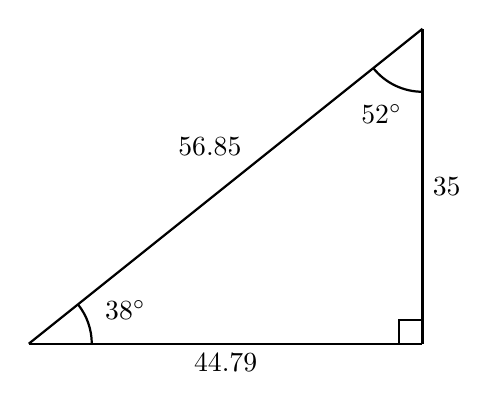
\begin{tikzpicture}[thick]
          \coordinate (A) at (0,1);
          \coordinate (B) at (5,5);
          \coordinate (C) at (5,1);

          \draw[black] (C) -- (B) node[midway, right]{$35$};
          \draw[black] (A) -- (C) node[midway, below]{$44.79$};
          \draw (4.7,1) |- ++(0.3,0.3);
          \draw[black] (A) -- (B);
          \draw[black] (2.3,3.5) node{$56.85$};

          \tkzMarkAngle[fill= orange,size=0.8cm,%
          opacity=1](A,B,C)
          \tkzLabelAngle[pos = 1.2](A,B,C){$52^{\circ}$}

          \tkzMarkAngle[fill= orange,size=0.8cm,%
          opacity=1](C,A,B)
          \tkzLabelAngle[pos = 1.3](C,A,B){$38^{\circ}$}

          \end{tikzpicture}
      \end{center}

    \item[\textit{Q36.}]  \text{ } 
      \begin{center}
          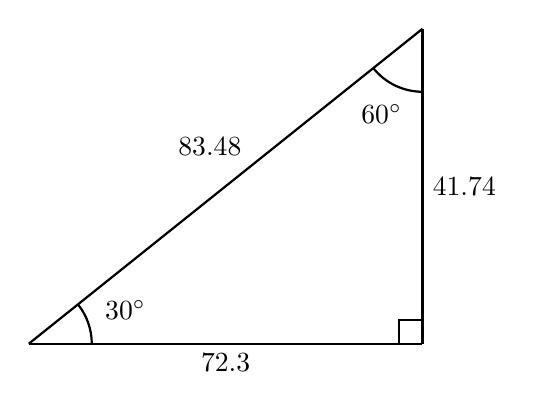
\begin{tikzpicture}[thick]
          \coordinate (A) at (0,1);
          \coordinate (B) at (5,5);
          \coordinate (C) at (5,1);

          \draw[black] (C) -- (B) node[midway, right]{$41.74$};
          \draw[black] (A) -- (C) node[midway, below]{$72.3$};
          \draw (4.7,1) |- ++(0.3,0.3);
          \draw[black] (A) -- (B);
          \draw[black] (2.3,3.5) node{$83.48$};

          \tkzMarkAngle[fill= orange,size=0.8cm,%
          opacity=1](A,B,C)
          \tkzLabelAngle[pos = 1.2](A,B,C){$60^{\circ}$}

          \tkzMarkAngle[fill= orange,size=0.8cm,%
          opacity=1](C,A,B)
          \tkzLabelAngle[pos = 1.3](C,A,B){$30^{\circ}$}

          \end{tikzpicture}
      \end{center}

  \end{itemize}
\end{qstn}

\newpage

\begin{qstn} \text{ }
  \begin{itemize} 
    \item[\textit{Q41.}] $x = 230.9$.
    \item[\textit{Q42.}] $x = 95.1$.
    \item[\textit{Q44.}] $x = 5.77$.
  \end{itemize}
\end{qstn}

\begin{qstn} \text{ }
  \begin{enumerate}[label=(\alph*)]
    \item $A_{\triangle ABC} = 3\left(6 + 6\sqrt{3} \right)$ square units.
    \item (This will be an assignment problem so I wont give the solution here)
      % $A_{\triangle SPQ} = \frac{169}{8} \left( 3 + \sqrt{3}\right)$ square units.
  \end{enumerate}
\end{qstn}










\end{document}




























